\subsection{Генерация модификаций трассы}

Для генерации трасс с консистентными потоками управления и данных, необходимо поддержать модификации для следующих данных трассы (см. раздел \ref{sec:execution_traces}):

\begin{itemize}
    \item Начальное регистровое состояние

    Начально регистровое состояние может содержать адреса, которые необходимо заменить в соответствии с картой перемещений.

    \item Обращения к памяти

    Обращения к памяти должны происходить по измененным адресам. Также, данные этих обращений могут сами по себе быть адресами.

    \item Значения регистров общего назначения

    Регистровые значения, используемые в качестве адресов, должны быть заменены.
\end{itemize}

Для упрощения задачи запретим добавлять записи типа "обращение в память" и модифицировать размеры и типы обращений для существующих записей: поток данных выходной трассы должен быть похож на исходный, но с замененными адресами. Таким образом, будут использованы четыре вида модификаций для записей трассы (три из которых генерируются на рассматриваемой стадии обработки):

\begin{itemize}
    \item Модификации начального регистрового состояния

    \item Модификации чтений из памяти

    \begin{itemize}
        \item Данные могут быть заменены, если из памяти читается значение, используемое в дальнейшем в качестве адреса.
        \item Адрес чтения должен быть получен из исходного с помощью карты перемещений.
        \item Новые записи не добавляются.
    \end{itemize}

    \item Модификации записей в память

    \begin{itemize}
        \item Данные получаются из симуляции: в память может записываться перемещенный адрес (возможно, преобразованный) или старые данные.
        \item Адрес записи должен быть получен из исходного с помощью карты перемещений.
        \item Новые записи не добавляются.
        \item Не генерируются на рассматриваемой стадии обработки: преобразования тривиальные и осуществляются при записи выходной трассы.
    \end{itemize}

    \item Модификации записей в регистры общего назначения

    \begin{itemize}
        \item Регистровые значения для существующих записей могут быть изменены.
        \item Могут быть добавлены новые записи, исправляющие потоки управления и данных.
    \end{itemize}
\end{itemize}

Генерация модификаций происходит в два этапа:

\begin{enumerate}
    \item Поиск адресов и смещений на ГПД

    На этом этапе производится поиск ребер, значения которых (возможно, после некоторых преобразований) используются в качестве адресов. Для найденных ребер генерируются первичные модификации трассы.

    \item Симуляционный проход по модифицированной трассе

    На этом этапе детектируются расхождения потока управления и потока данных симулятора с ожидаемым поведением на модифицированной трассе. При детектировании расхождений генерируются вторичные модификации трассы, исправляющие ошибки.
\end{enumerate}

Предложенный алгоритм по построению поддерживает любые паттерны адресации в трассе, но может генерировать трассы с большим количеством компенсаций. Подробнее свойства предложенного алгоритма будут рассмотрены в дальнейшем.

\subsubsection{Поиск адресов и смещений}

Введем два маркера для ребер ГПД: красный маркер отмечает ребра, обработанные в ходе обратного обхода ГПД; зеленый маркер отмечает ребра, попавшие в очередь прямого обхода ГПД. В данную очередь будем помещать только ребра, еще не покрашенные зеленым маркером.

Будем называть два ребра близкими по значению если абсолютная разность их значений меньше некоторого порогового значения, являющегося гиперпараметром решения (обозначим как ADDR\_SIMILARITY\_THRESHOLD). Также будем называть ребро $e \in F \subseteq E$ ближайшим по значению к ребру $g$ среди ребер $F$, если $e$ и $g$ близки по значению и пара $(e, g)$ обладает минимальной абсолютной разностью значений среди всех пар $F \times \{g\}$.

Сначала с ГПД собираются ребра, значения которых используются целевыми инструкциями в качестве адресов или считаются адресами по другим косвенным признакам (\glsdisp{addr_edge}{адресные ребра}). К таким значениям относятся: базовые адреса обращений в память; адреса переходов потока управления; адреса, используемые для операций с кешами; значения, которые сравниваются с адресами или вычитаются из них; и т.п.

Для каждого адресного ребра, строится обратный путь на ГПД, начинающийся с этого ребра. Построение выполняется последовательно. На каждом шаге для текущего конечного ребра пути (обозначим это ребро как $e$) выбирается следующее ребро из множества рёбер, входящих в начальную вершину $e$. Построение пути осуществляется до выполнения одного из условий останова: достижения псевдо-инструкции; ошибки поиска следующего ребра; достижения ребра, окрашенного красным маркером; и т.п. Конечное ребро построенного пути будем называть \glsdisp{src_addr_edge}{исходным адресным ребром}. Для таких ребер, а также ребер пути с локациями в памяти, генерируются первичные модификации трассы, что позволяет заменить больш\'{у}ю часть используемых адресов (так как изменения будут распространяться по потоку данных) путем малого количества модификаций трассы. Все ребра построенного пути красятся красным маркером, а исходные адресные ребра также помещаются в очередь прямого обхода ГПД (если они еще не окрашены зеленым маркером). Блок схема алгоритма построения обратных путей на ГПД представлена на рис. \ref{fig:addr_source_search}.

\begin{figure}[h!]
    \centering
    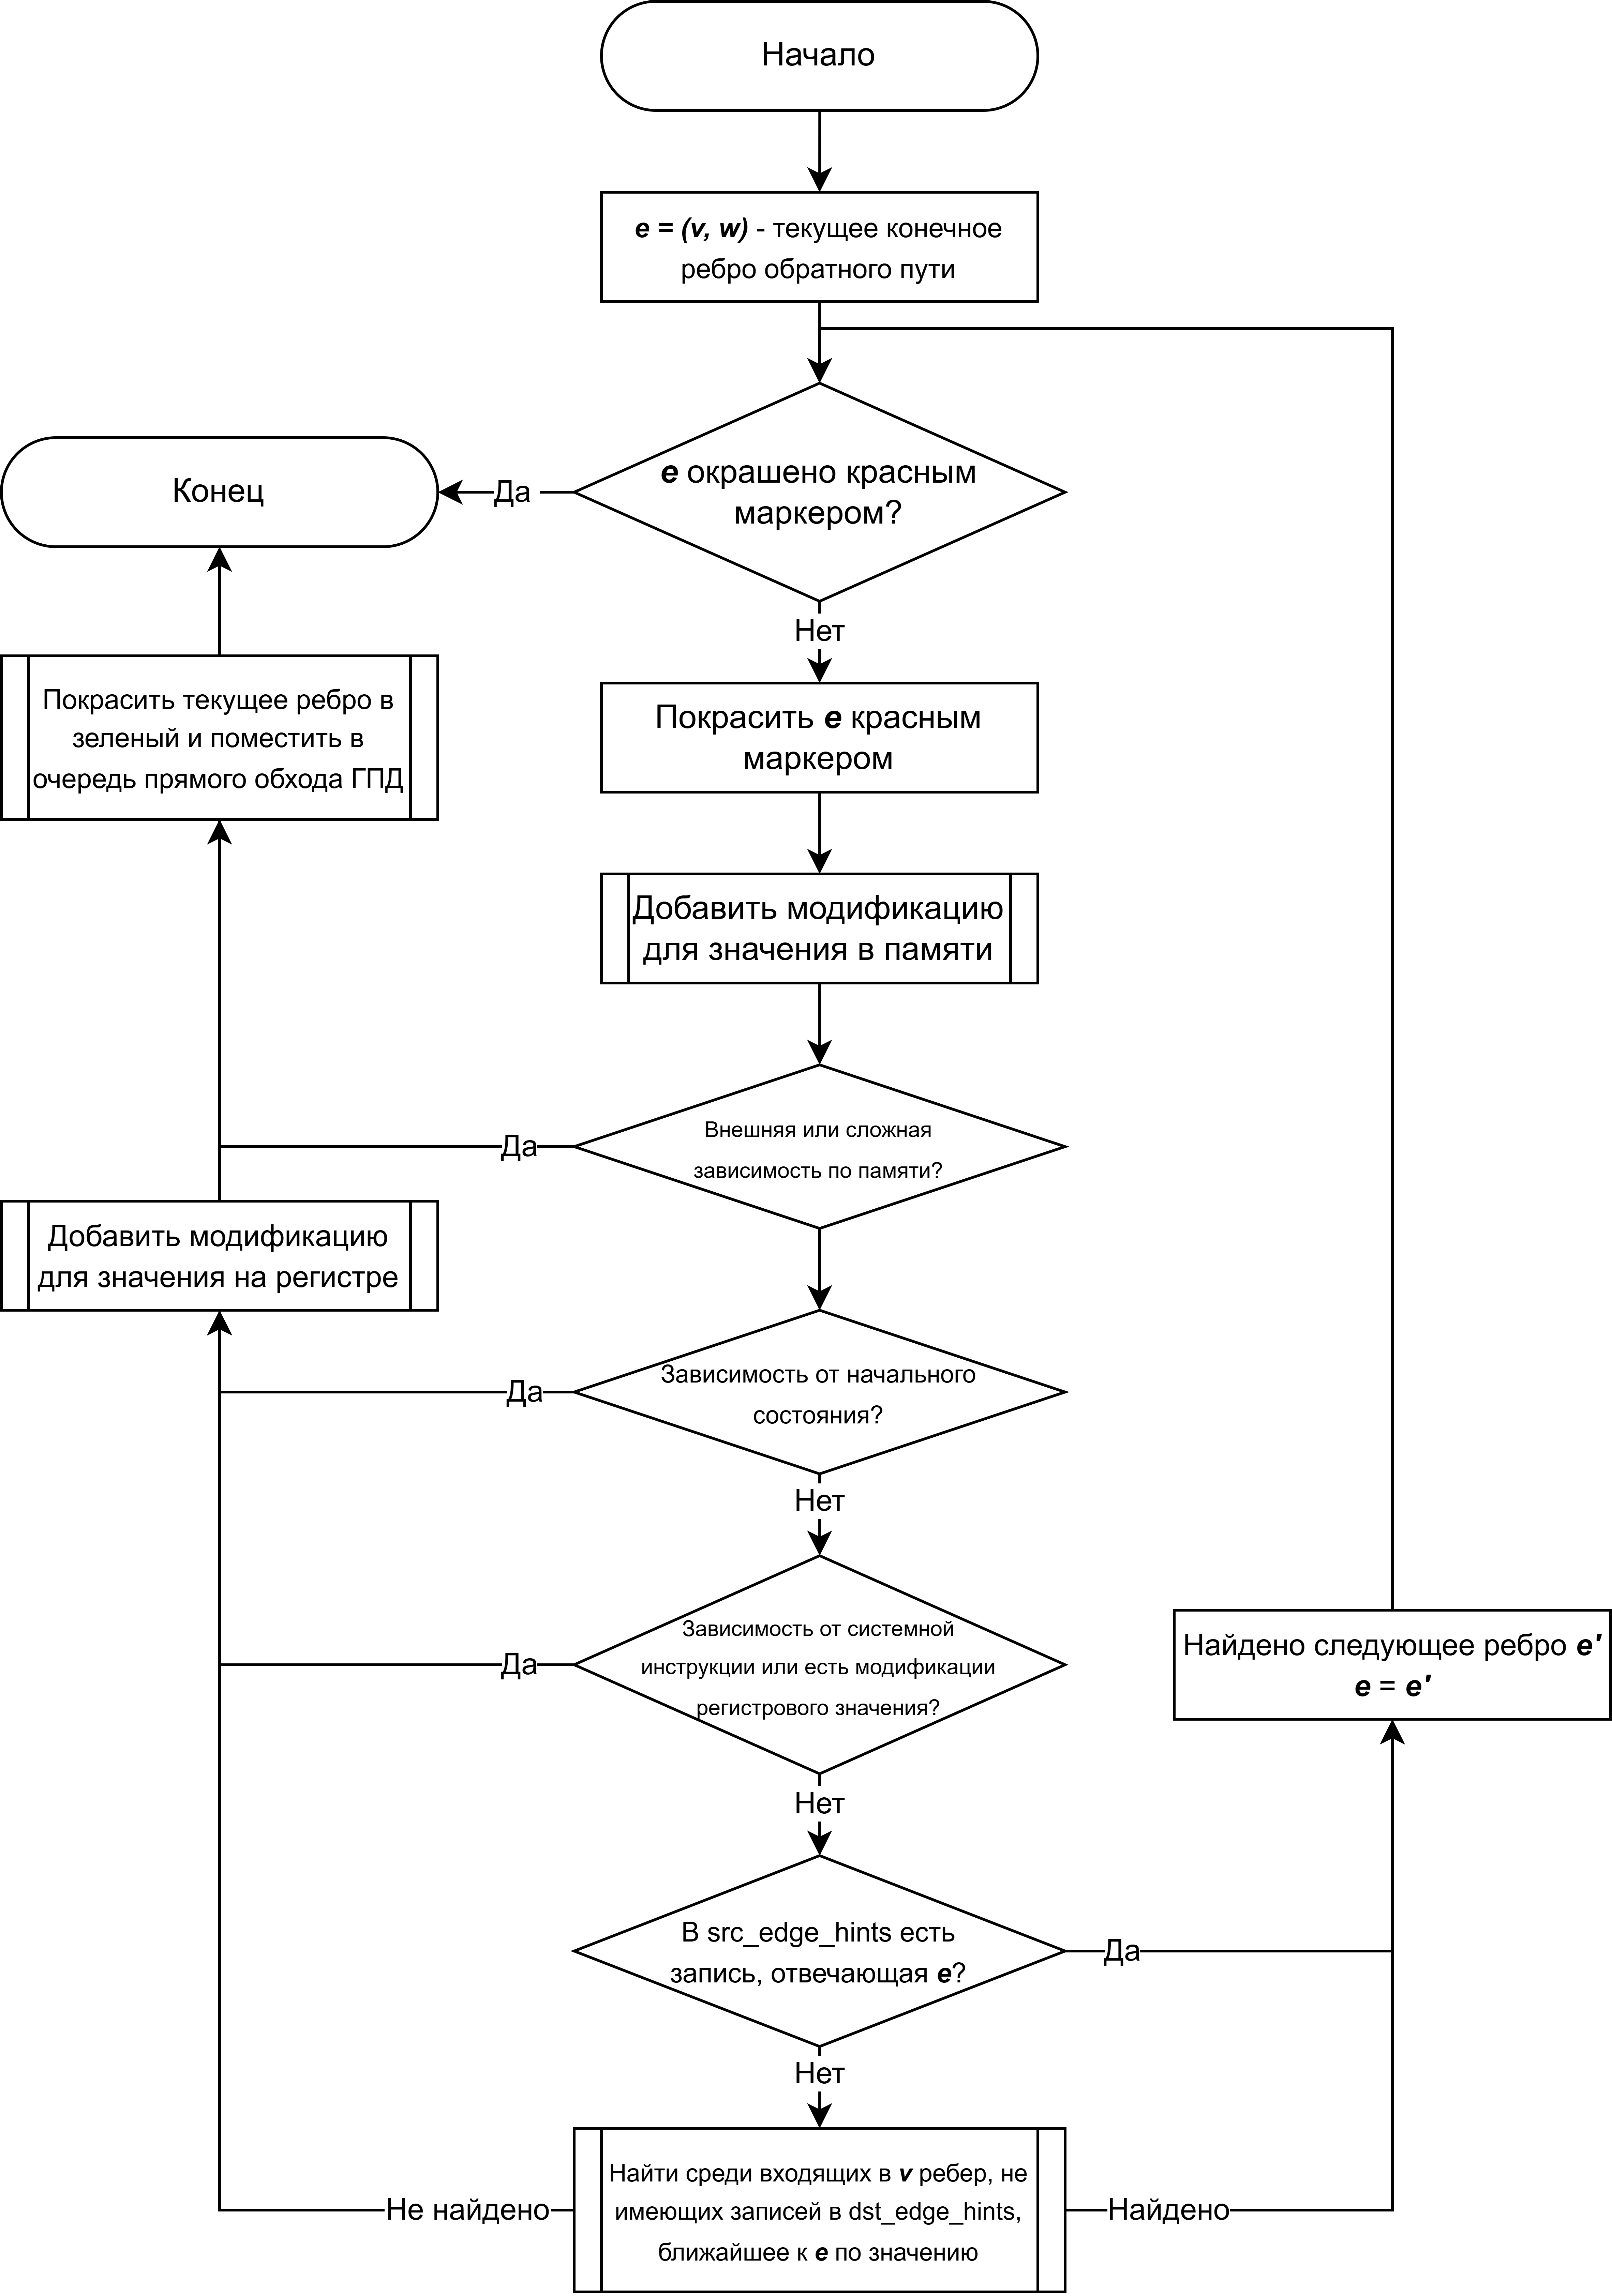
\includegraphics[width=0.8\linewidth]{pics/addr_source_search.drawio.png}
    \caption{Блок схема алгоритма построения обратных путей на ГПД.}
    \label{fig:addr_source_search}
\end{figure}

Затем производится обработка ребер в очереди прямого обхода ГПД. Для каждого ребра $e$ строится обратный путь (если он еще не был построен) и осуществляется поиск ребер для дальнейшего обхода. Найденные ребра добавляются в очередь прямого обхода:

\begin{itemize}
    \item Ребра с такой же начальной вершиной и локацией

    \item Ребра, значения которых сравниваются со значением $e$

    Если $e$ входит в вершину $v$, являющуюся инструкцией сравнения, то все входные ребра $v$ добавляются в очередь.

    \item Ребра, значения которых участвуют в вычитании со значением $e$

    Сценарий аналогичен предыдущему, но значения добавляемых ребер должны быть больше некоторого порогового значения, являющегося гиперпараметром решения (обозначим как ADDR\_MIN\_VALUE).

    \item Ребра, соответствующие $e$ в dst\_edge\_hints.

    \item Ребра, выходящие из $v$, близкие по значению к $e$

    Данные ребра добавляются только если для $e$ нет записей в dst\_edge\_hints.
\end{itemize}

\FloatBarrier

Прямой обход ГПД позволяет найти дополнительные адресные ребра для построения обратных путей на графе и генерации первичных модификаций. Этот обход нужен, так как часть значений в трассе может не использоваться в качестве адресов напрямую, но может сравниваться с адресами, использоваться для подсчета хеш сумм адресов, и т. п. Часть таких значений будет найдена при данном обходе, что позволит в дальнейшем сделать меньше вторичных модификаций (которые всегда снижают репрезентативность трассы).

\subsubsection{Симуляционный проход по модифицированной трассе} \label{sec:patched_trace_sim}

На данной стадии производится проход по трассе, аналогичный изображенному на рис. \ref{fig:trace_simulation}. Но записи трассы преобразуются в соответствии со сгенерированными модификациями. Также до и после каждого симуляционного шага потоки управления и данных симулятора проверяются на расхождения с ожидаемым поведением. При детектировании расхождения, состояние симулятора исправляется и генерируются вторичные модификации трассы, соответствующие исправлению. В случае расхождения после симуляционного шага, состояние симулятора восстанавливается и шаг делается повторно (с примененными исправлениями). Описанный подход позволяет генерировать трассы с консистентными потоками управления и данных. Блок схема алгоритма представлена на рис. \ref{fig:patched_trace_sim}.

\begin{figure}[h!]
    \centering
    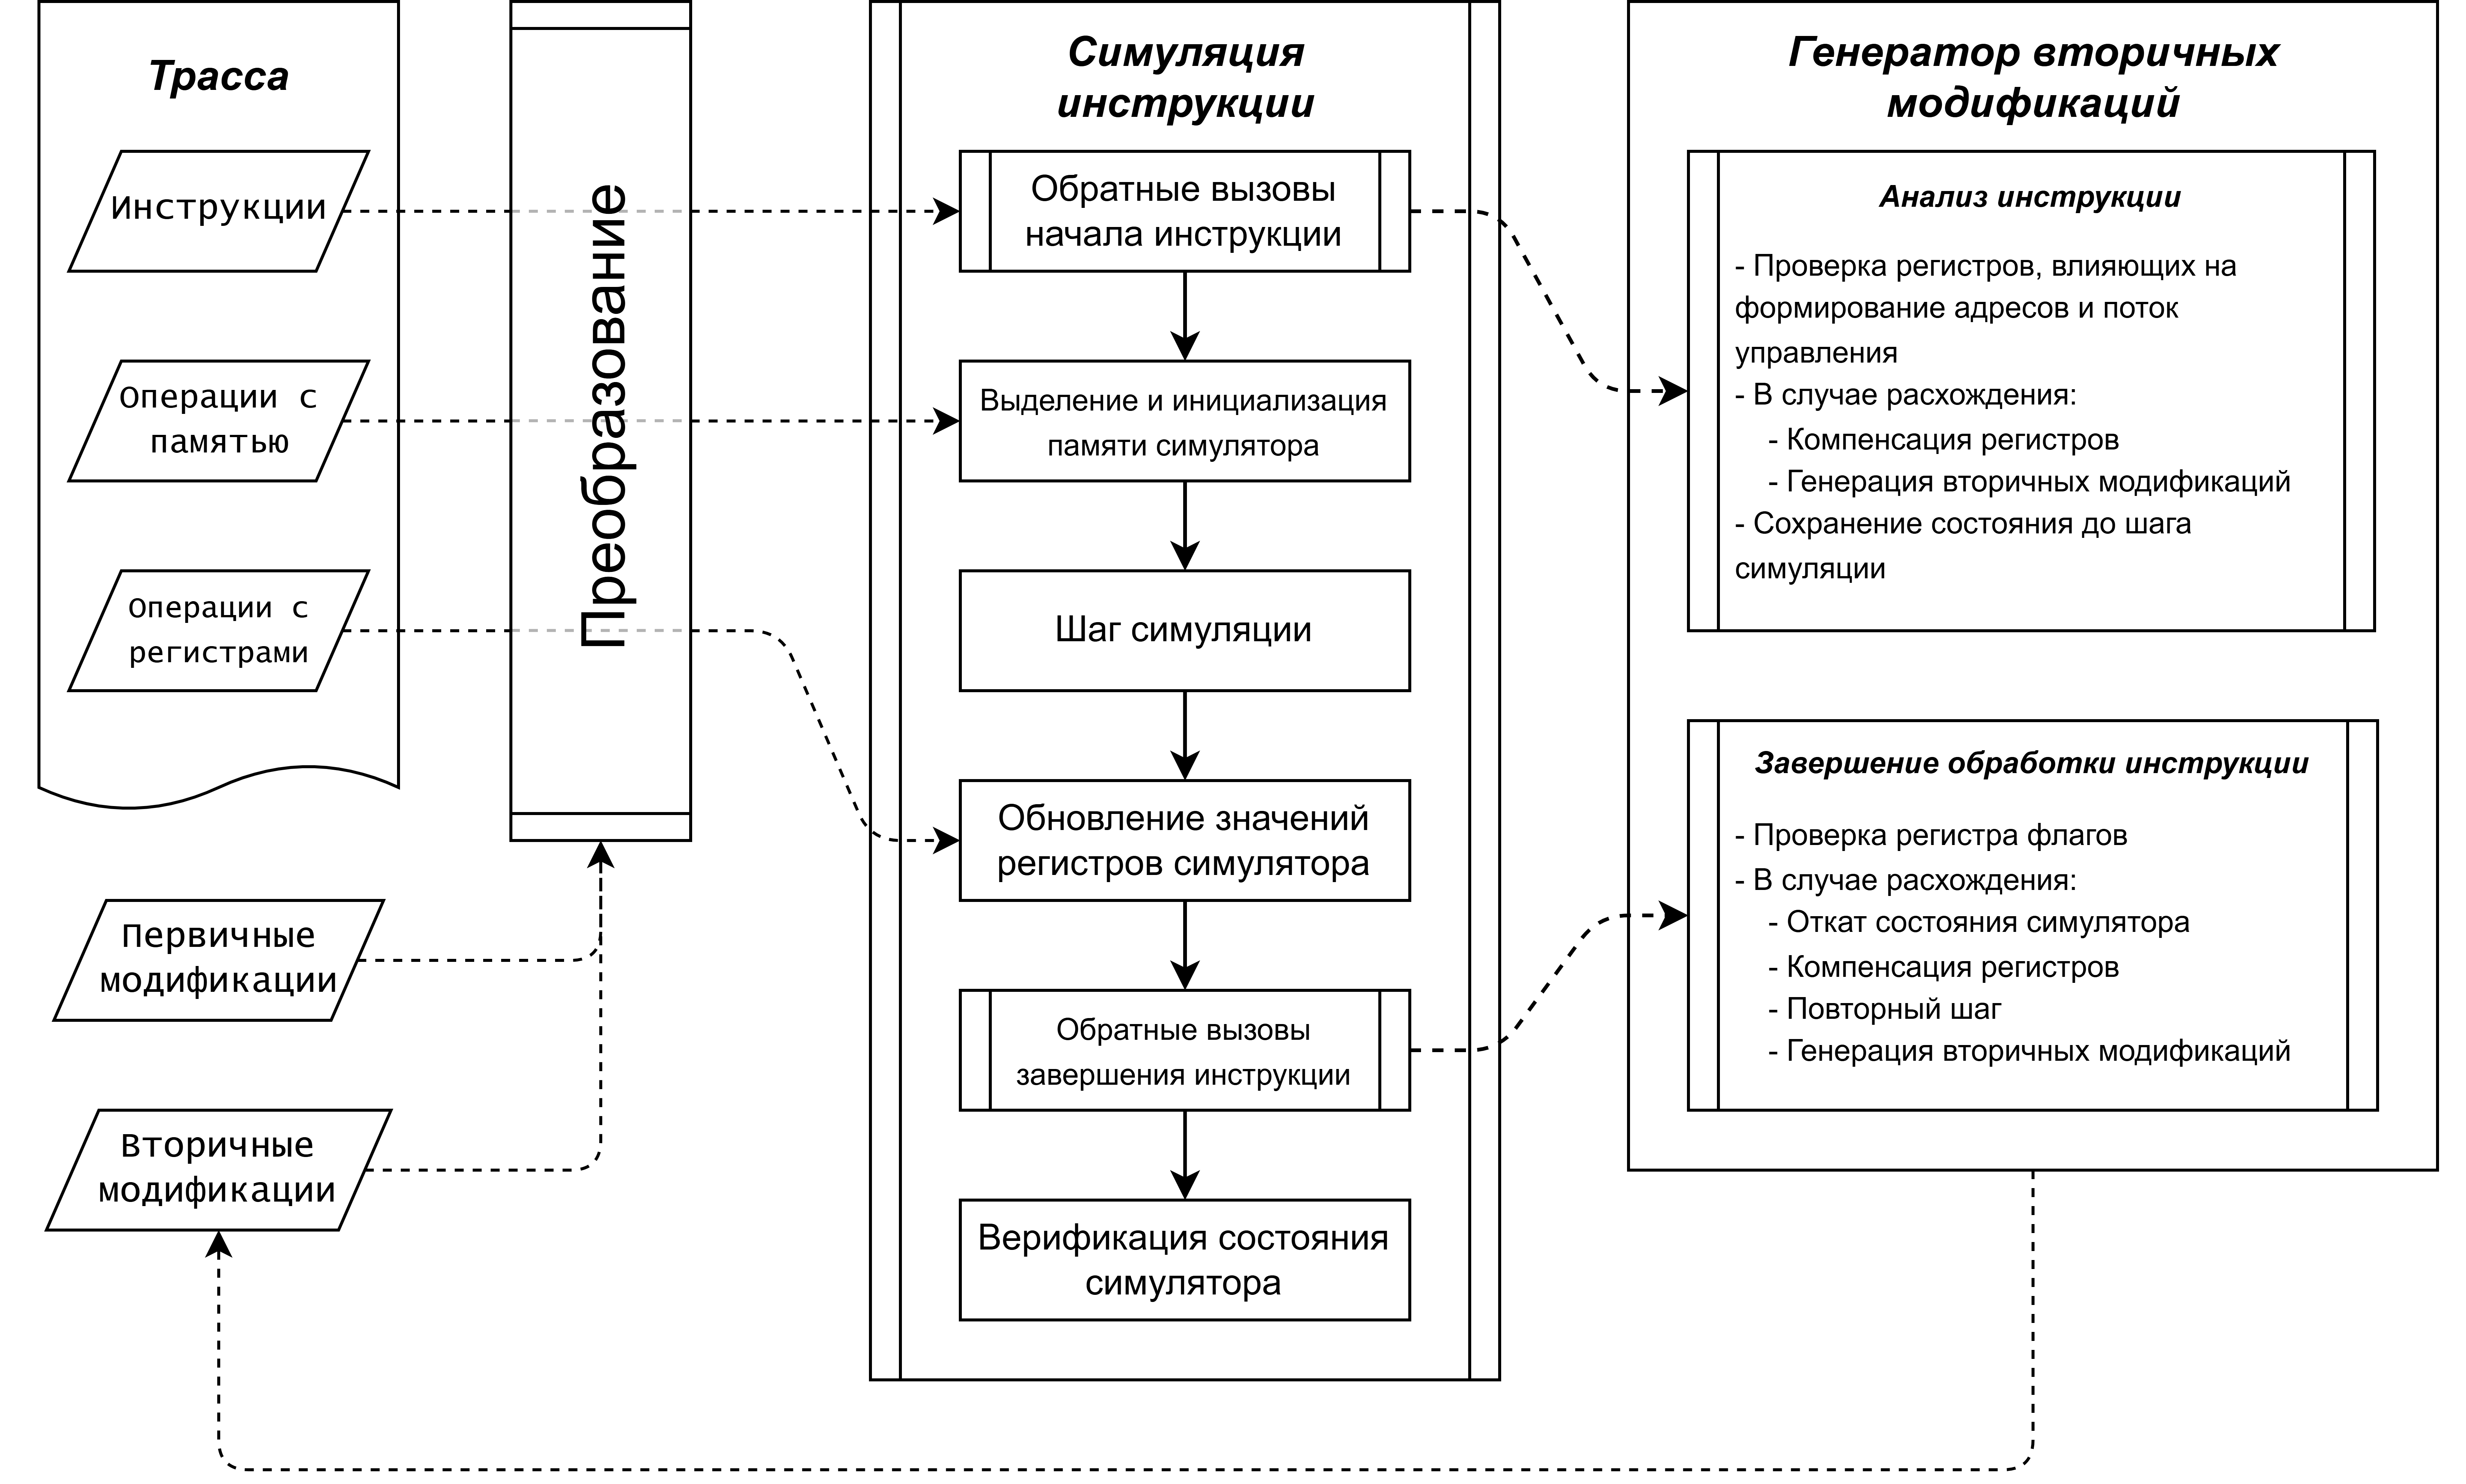
\includegraphics[width=\linewidth]{pics/patched_trace_sim.drawio.png}
    \caption{Блок схема симуляционного прохода по модифицированной трассе.}
    \label{fig:patched_trace_sim}
\end{figure}

\FloatBarrier
